\section{Image Approximation using the ROF Model} % (fold)
\label{sec:image_approximation_using_the_rof_model}
    
    In this section we show some approximations of input images. Besides we compare run-time and different parameters. We also provide the best estimates of parameters for each model. Further, we proof that using the Lagrange Multiplier method for the convex relaxed Mumford-Shah model leads to a run-time speed up of a factor 450 compared with the proposed method in \cite{Pock-et-al-iccv09}.

    % % \subsubsection{Image Approximation using the ROF Model} % (fold)
    % % \label{sub:image_approximation_using_the_rof_model}
        
    % We start our comparison by considering the ROF model. In this model we minimized the energy
    %     $$
    %         E_{ROF}(u) = \frac{\lambda}{2} ||u - g||_{2}^{2} + ||\nabla u||_{1}.
    %     $$
    % After rewriting this into a saddle-point formulation we derived
    %     $$
    %         \min_{u \in X} \max_{p \in Y} \langle \nabla u, p \rangle - \delta_{P}(p) + \frac{\lambda}{2}||u - g||_{2}^{2}.
    %     $$
    % For the sake of completeness, the corresponding proximity operators of this model where computed as
    %     $$
    %         p = (\textnormal{Id} + \sigma\,\partial\,F^{\ast})^{-1}(\tilde{p}) = \Pi_{P}(\tilde{p}) \Longleftrightarrow p_{i,j} = \frac{\tilde{p}_{i, j}}{\max(1, |\tilde{p}_{i, j}|)},
    %     $$
    % and
    %     $$
    %         u = (\textnormal{Id} + \tau\,\partial\,G)^{-1}(\tilde{u}) \Longleftrightarrow u_{i,j} = \frac{\tilde{u}_{i,j} + \tau\lambda g}{1 + \tau\sigma},
    %     $$
    % for all $i = 1, ..., N$ and $j = 1, ..., M$.

    The implementation for this model using the proposed primal-dual algorithm \ref{alg:fast_primal_dual_algorithm} is straightforward. %Recalling the algorithm we had:

    % \begin{algorithm}[First-Order Primal-Dual Algorithm]
    %     Choose $(u^{0}, p^{0}) \in X \times Y$ and let $\bar{u}^{0} = u^{0}$. Further let $\tau, \sigma > 0$ with $\sigma\tau L^{2} \le 1$ and $\theta \in [0, 1]$. Then, we let for each $n \ge 0$
    %         \begin{equation}
    %             \left\{ 
    %                 \begin{array}{l l}
    %                     p^{n+1} = (\textnormal{Id} + \sigma\,\partial\,F^{\ast})^{-1}(p^{n} + \sigma\,K\bar{u}^{n}) \\
    %                     u^{n+1} = (\textnormal{Id} + \tau\,\partial\,G)^{-1}(u^{n} - \tau\,K^{\ast}p^{n+1}) \\
    %                     \bar{u}^{n+1} = u^{n+1} + \theta (u^{n+1} - u^{n}).
    %                 \end{array}
    %             \right.
    %         \end{equation}
    % \end{algorithm}

    \subsection{Implementation Issues} % (fold)
    \label{sub:implementation_issues}
        
        In our framework we propose both, a C++ and a CUDA implementation. Since, there is no big difference in the code itself, we discuss the implementation not programming language specific. We set $K = \nabla$ with the proposed discretization stated in section \ref{sec:discrete_setting}. Further, we consider $u$, $\bar{u}$, etc. being accessed with $u_{i,j,k}$. For the approximation of color images we have that $k = 1, 2, 3$, in the case of grayscaled images $k = 1$.\\

        \subsubsection{Initialization}
        \label{sub:initialization}

            According to \cite{Chambolle10afirst-order} the algorithm is independent of its initialization. The better the initialization at the beginning, the faster the convergence to a optimal solution. We ran numerous tests to find good initialization values, e.g. setting everything to zero or using the maximal value $255$. It turned out, that the best choice is the input image $g$ itself. In table \ref{tab:init_compare} we show a few estimates of our tests. So, overall we initialize with $p = 0$ and $u = g$.

            \begin{center}
                \begin{tabular}{| l | l | l |}
                \hline
                Initialization & Iterations & CPU time \\ \hline\hline
                0 & 593 & 5.13 \\ \hline
                124 & 575 & 4.88 \\ \hline
                255 & 562 & 4.84 \\ \hline
                $g$ & 510 & 4.22 \\ \hline
                \end{tabular}
                \label{tab:init_compare}
            \end{center}

        \subsubsection{Computing $p^{n+1} = (\textnormal{Id} + \sigma\,\partial\,F^{\ast})^{-1}(p^{n} + \sigma\,\nabla\bar{u}^{n})$}
        \label{sub:computing_p}

            In the $n+1$-th iteration step we first need to estimate the gradient of $\bar{u}^{n}$. For this we allocate two variables $dx$ and $dy$ and compute under the premise that we discretized $\nabla$ by forward differences with Neumann boundary conditions
                $$
                    dx = \bar{u}_{i+1,j,k} - \bar{u}_{i,j,k} \,\,\,\,\, \textnormal{and} \,\,\,\,\, dy = \bar{u}_{i,j+1,k} - \bar{u}_{i,j,k},
                $$
            where we set $dx = 0$ if $i + 1 < M$ and $dy = 0$ if $j + 1 < N$.
            After that, we multiply both values with $\sigma$ and then add the old estimate of $p$, namely $p^{n}$ to them. This means
                $$
                    dx = dx + p_{x_{i,j,k}}^{n} \,\,\,\,\, \textnormal{and} \,\,\,\,\, dy = dy + p_{y_{i,j,k}}^{n}.
                $$
            At the end we only need to apply the proximity operator of the function $F^{\ast}$ to the variables $dx$ and $dy$ and save the observed value in $p^{n+1}$. We compute
                $$
                    p_{x_{i,j,k}}^{n+1} = \frac{dx}{\max(1, |dx|)} \,\,\,\,\, \textnormal{and} \,\,\,\,\, p_{y_{i,j,k}}^{n+1} = \frac{dy}{\max(1, |dy|)}.
                $$
            \begin{algorithm}[Dual Ascent]
            \label{alg:dual_ascent}
                Summarizing this procedure in a function, we get
                \begin{lstlisting}
template<typename T>
void dual_asc(T* p_x, T* p_y, T* u_bar, float sigma, int M, int N, int C) {
  T dx, dy;
  int index;
  for (int k = 0; k < C; k++) {
    for (int i = 0; i < M; i++) {
      for (int j = 0; j < N; j++) {
        index = j + i * N + k * M * N;
        dx = i+1<M ? u_bar[j + (i+1) * N + k * M * N]-u_bar[index] : 0;
        dy = j+1<N ? u_bar[(j+1) + i * N + k * M * N]-u_bar[index] : 0;
        dx = p_x[index] + sigma * dx;
        dy = p_y[index] + sigma * dy;
        p_x[index] = dx / fmax(1.f, fabs(dx));
        p_y[index] = dy / fmax(1.f, fabs(dy));
      }
    }
  }
}
                \end{lstlisting}
                where $C$ is the number of color channels and the template value $T$ is mostly used as float.
            \end{algorithm}

        These 18 lines of code are used to compute the update on $p^{n+1}$. To be able to use this function in another framework, like for minimizing the TVL1 energy, we only need to change the last two lines in the for-loops. These resemble the proximity operator and this operator can vary from model to model.\\

        \subsubsection{Computing $u^{n+1} = (\textnormal{Id} + \tau\,\partial\,G)^{-1}(u^{n} - \tau\,\textnormal{div}p^{n+1})$}
        \label{sub:computing_u}

            The first thing to mention for this line of pseudo code is, that we set $\nabla^{T} = -\textnormal{div}$. But then we compute
                $$
                    u^{n+1} = (\textnormal{Id} + \tau\,\partial\,G)^{-1}(u^{n} + \tau\,\nabla^{T}p^{n+1}).
                $$

            We follow the same procedure as before: we allocate values $dx$, $dy$ and this time also $sum$, in which we store the sum of the partial derivatives. Using backward differences with Dirichlet boundary conditions, like in definition \ref{def:discrete_divergence_operator}, we compute
                $$
                    dx = p_x{i,j,k} - p_x{i-1,j,k}, \,\,\, dy = p_y{i,j,k} - p_y{i,j-1,k} \,\,\, \textnormal{and} \,\,\, sum = \tau \cdot (dx + dy).
                $$
            And we additional take into account that if $i + 1 < M$ or $j + 1 < N$ we have
                $$
                    dx = -p_x{i-1,j,k} \,\,\,\,\, \textnormal{or} \,\,\,\,\, dy = -p_y{i,j-1,k}
                $$
            and if $i > 0$ or $j > 0$ we compute
                $$
                    dx = p_x{i,j,k} \,\,\,\,\, \textnormal{or} \,\,\,\,\, dy = p_y{i,j,k}.
                $$
            As we already multiplied the discrete divergence with the parameter $\tau$, it is left to add the previous estimate $u^{n}$ by
                $$
                    sum = u_{i,j,k} + sum.
                $$
            In a last step we apply the proximity operator for the function $G$ and observe
                $$
                    u_{i,j,k}^{n+1} = \frac{sum + \tau\lambda g_{i,j,k}}{1 + \tau\sigma}.
                $$
                \begin{algorithm}[Primal Descent]
                \label{alg:primal_descent}
                    Summarizing again in a function, we have
                    \begin{lstlisting}
    template<typename T>
    void primal_desc(T* p_x, T* p_y, T* u, T* g, float tau, float lambda, int M, int N, int C) {
      T dx, dy, sum;
      int index;
      for (int k = 0; k < C; k++) {
        for (int i = 0; i < M; i++) {
          for (int j = 0; j < N; j++) {
            index = j + i * N + k * M * N;
            dx = (i+1<M ? p_x[index] : 0.f) -
                 (i>0 ? p_x[j + (i-1) * N + k * M * N] : 0.f);
            dy = (j+1<N ? p_y[index] : 0.f) -
                 (i>0 ? p_y[(j-1) + i * N + k * M * N] : 0.f);
            sum = tau * (dx + dy);
            sum += u[index];
            u[index] = (sum + tau * lambda * g[index]) / (1.f + tau * lambda);
          }
        }
      }
    }
                    \end{lstlisting}
                    where $C$ is the number of color channels and the template value $T$ is mostly used as float.
                \end{algorithm}

            It is only left to compute the extrapolation step. This is a straightforward computation, since we just add vectors.

                \begin{algorithm}[Extrapolation]
                \label{alg:extrapolation}
                    In a function we have
                    \begin{lstlisting}
    template<typename T>
    void extrapolation(T* u_bar, T* u, T* u_prev, float theta, int M, int N, int C) {
      for (int i = 0; i < N*M*C; i++) {
        u_bar[i] = u[i] + theta * (u[i] - u_prev[i]);
        u_prev[i] = u[i];
      }
    }
                    \end{lstlisting}
                    where $C$ is the number of color channels and the template value $T$ is mostly used as float.
                \end{algorithm}

            We also set $u_{prev}$ to the current estimate $u$, because we need this in each step of the extrapolation function. As a last function we provide the primal-dual algorithm, which makes use of the stated functions:

                \begin{algorithm}[Primal-Dual Algorithm]
                \label{alg:primal_dual}
                    In a function we have
                    \begin{lstlisting}
template<typename T>
void ROF(T* u, T* g, float lambda, float tau, int M, int N, int C) {
  float sigma = 1.f / (tau * 8.f);
  float theta = 2.f;
  T* u_bar = new T[M*N*C];
  T* u_prev = new T[M*N*C];
  T* p_x = new T[M*N*C];
  T* p_y = new T[M*N*C];
  
  void dual_asc(p_x, p_y, u_bar, sigma, M, N, C);
  void primal_desc(p_x, p_y, u, g, tau, lambda, M, N, C);
  void extrapolation(u_bar, u, u_prev, theta, M, N, C);

  delete [] u_bar;
  delete [] u_prev;
  delete [] p_x;
  delete [] p_y;
}
                    \end{lstlisting}
                    where $C$ is the number of color channels and the template value $T$ is mostly used as float.
                \end{algorithm}

            We derive the computation of $\sigma$, because of the convergence theorem \ref{the:primal_dual_convergence}. It states, that we have a convergent algorithm if $\sigma\tau L^{2} < 1$. For that we get
                $$
                    \sigma = \frac{1}{\tau * L^{2}} = \frac{1}{\tau * 8},
                $$
            by proposition \ref{prop:bound_on_the_norm}. Further, we set $\theta = 2$ to derive the version suggested in \cite{Chambolle10afirst-order}.

            Now, that we know how the implementation of the ROF model can be done, we want to compare some outcomes of the algorithm. We ran two separate parameter estimations: first we looked for the perfect $\lambda$ for a minimal energy, a fast convergence and a visible good approximation $u$. Afterwards, we estimated the $\tau$, for which the algorithm converges quickly with respect to the optimal $\lambda$. In figure \ref{fig:rof_lena_first_compare} one can see the evolution of the Lena image using different parameters $\lambda$ and estimating the perfect fit.

        % \begin{figure}[ht]
        %     \centering
        %     \begin{subfigure}[b]{0.4\textwidth}
        %         \includegraphics[width=\textwidth]{img/approximation/rof/006lena.png}
        %         \caption{$\lambda = 0.06$}
        %     \end{subfigure}
        %     \begin{subfigure}[b]{0.4\textwidth}
        %         \includegraphics[width=\textwidth]{img/approximation/rof/007lena.png}
        %         \caption{$\lambda = 0.07$}
        %     \end{subfigure}
        %     \begin{subfigure}[b]{0.4\textwidth}
        %         \includegraphics[width=\textwidth]{img/approximation/rof/009lena.png}
        %         \caption{$\lambda = 0.09$}
        %     \end{subfigure}
        %     \begin{subfigure}[b]{0.4\textwidth}
        %         \includegraphics[width=\textwidth]{img/approximation/rof/01lena.png}
        %         \caption{$\lambda = 0.1$}
        %     \end{subfigure}
        %     \begin{subfigure}[b]{0.4\textwidth}
        %         \includegraphics[width=\textwidth]{img/approximation/rof/06lena.png}
        %         \caption{$\lambda = 0.6$}
        %     \end{subfigure}
        %     \begin{subfigure}[b]{0.4\textwidth}
        %         \includegraphics[width=\textwidth]{img/approximation/rof/09lena.png}
        %         \caption{$\lambda = 0.9$}
        %     \end{subfigure}
        %     \caption{Approximation of the Lena image with the ROF Model. Again, the higher $\lambda$ the closer the outcome of the algrithm to the original image.}
        % \label{fig:rof_lena_compare}
        % \end{figure}

    \subsection{Best $\lambda$ estimation}
    \label{sub:best_lambda_estimation_rof}

        To estimate the possible best $\lambda$ we started by testing all values in the range from $0.001$ to $0.01$ by adding in each approximation a factor $0.001$ to the parameter $\lambda$. In figure \ref{fig:rof_lena_first_compare} one can see, that an increasing value for $\lambda$ makes the image more visible. But, it turned out that the algorithm took a long time till convergence - differing from over 1000 to almost 6000 iterations. Additionally, the PSNR is then between 18 and 25, which is too bad for a good approximation of an image.

        \begin{figure}[ht]
            \centering
            \begin{subfigure}[b]{0.18\textwidth}
                \includegraphics[width=\textwidth]{img/approximation/rof/rof_start/0001lena.png}
                \caption{$\lambda = 0.001$}
            \end{subfigure}
            \begin{subfigure}[b]{0.18\textwidth}
                \includegraphics[width=\textwidth]{img/approximation/rof/rof_start/0002lena.png}
                \caption{$\lambda = 0.002$}
            \end{subfigure}
            \begin{subfigure}[b]{0.18\textwidth}
                \includegraphics[width=\textwidth]{img/approximation/rof/rof_start/0003lena.png}
                \caption{$\lambda = 0.003$}
            \end{subfigure}
            \begin{subfigure}[b]{0.18\textwidth}
                \includegraphics[width=\textwidth]{img/approximation/rof/rof_start/0004lena.png}
                \caption{$\lambda = 0.004$}
            \end{subfigure}
            \begin{subfigure}[b]{0.18\textwidth}
                \includegraphics[width=\textwidth]{img/approximation/rof/rof_start/0005lena.png}
                \caption{$\lambda = 0.005$}
            \end{subfigure}
            \begin{subfigure}[b]{0.18\textwidth}
                \includegraphics[width=\textwidth]{img/approximation/rof/rof_start/0006lena.png}
                \caption{$\lambda = 0.006$}
            \end{subfigure}
            \begin{subfigure}[b]{0.18\textwidth}
                \includegraphics[width=\textwidth]{img/approximation/rof/rof_start/0007lena.png}
                \caption{$\lambda = 0.007$}
            \end{subfigure}
            \begin{subfigure}[b]{0.18\textwidth}
                \includegraphics[width=\textwidth]{img/approximation/rof/rof_start/0008lena.png}
                \caption{$\lambda = 0.008$}
            \end{subfigure}
            \begin{subfigure}[b]{0.18\textwidth}
                \includegraphics[width=\textwidth]{img/approximation/rof/rof_start/0009lena.png}
                \caption{$\lambda = 0.009$}
            \end{subfigure}
            \begin{subfigure}[b]{0.18\textwidth}
                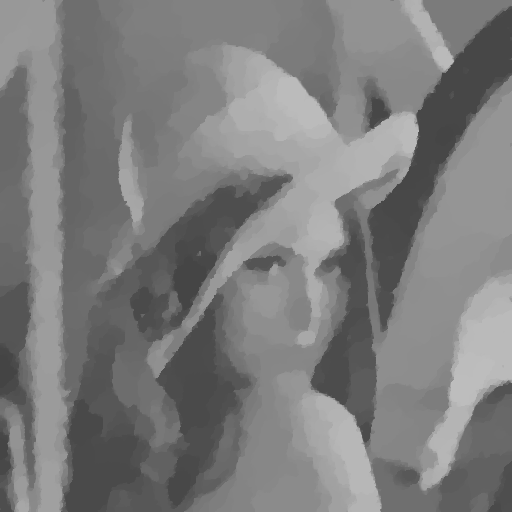
\includegraphics[width=\textwidth]{img/approximation/rof/rof_start/001lena.png}
                \caption{$\lambda = 0.01$}
            \end{subfigure}
            \caption{Approximation of the Lena image with the ROF Model. Again, the higher $\lambda$ the closer the outcome of the algrithm to the original image.}
        \label{fig:rof_lena_first_compare}
        \end{figure}

        It seemed not to be appropriable to go one one-thousandth steps and we already learned, that a small parameter does not lead to the desired results. We then turned our interest to the other extrem setting. We used the range from $0.1$ to $1$ in one-tenth steps. It not only lead to the perfect fit, it also produced good approximations $u$ of our input image $g$. This can also be seen in figure \ref{fig:rof_lena_second_compare}. We also want to show the table with some data like PSNR, iterations, energy and run-time.

        \begin{figure}[ht]
            \centering
            \begin{subfigure}[b]{0.18\textwidth}
                \includegraphics[width=\textwidth]{img/approximation/rof/rof_start/01lena.png}
                \caption{$\lambda = 0.1$}
            \end{subfigure}
            \begin{subfigure}[b]{0.18\textwidth}
                \includegraphics[width=\textwidth]{img/approximation/rof/rof_start/02lena.png}
                \caption{$\lambda = 0.2$}
            \end{subfigure}
            \begin{subfigure}[b]{0.18\textwidth}
                \includegraphics[width=\textwidth]{img/approximation/rof/rof_start/03lena.png}
                \caption{$\lambda = 0.3$}
            \end{subfigure}
            \begin{subfigure}[b]{0.18\textwidth}
                \includegraphics[width=\textwidth]{img/approximation/rof/rof_start/04lena.png}
                \caption{$\lambda = 0.4$}
            \end{subfigure}
            \begin{subfigure}[b]{0.18\textwidth}
                \includegraphics[width=\textwidth]{img/approximation/rof/rof_start/05lena.png}
                \caption{$\lambda = 0.5$}
            \end{subfigure}
            \begin{subfigure}[b]{0.18\textwidth}
                \includegraphics[width=\textwidth]{img/approximation/rof/rof_start/06lena.png}
                \caption{$\lambda = 0.6$}
            \end{subfigure}
            \begin{subfigure}[b]{0.18\textwidth}
                \includegraphics[width=\textwidth]{img/approximation/rof/rof_start/07lena.png}
                \caption{$\lambda = 0.7$}
            \end{subfigure}
            \begin{subfigure}[b]{0.18\textwidth}
                \includegraphics[width=\textwidth]{img/approximation/rof/rof_start/08lena.png}
                \caption{$\lambda = 0.8$}
            \end{subfigure}
            \begin{subfigure}[b]{0.18\textwidth}
                \includegraphics[width=\textwidth]{img/approximation/rof/rof_start/09lena.png}
                \caption{$\lambda = 0.9$}
            \end{subfigure}
            \begin{subfigure}[b]{0.18\textwidth}
                \includegraphics[width=\textwidth]{img/approximation/rof/rof_start/1lena.png}
                \caption{$\lambda = 1$}
            \end{subfigure}
            \caption{Approximation of the Lena image with the ROF Model. Again, the higher $\lambda$ the closer the outcome of the algrithm to the original image.}
        \label{fig:rof_lena_second_compare}
        \end{figure}

        Having a PSNR over 40 means, that we are extremely close to the original image. As discussed before, an image consists of data and noise and we seek to remove that noise from our images. We assumed to only consider approximation $u$, which have a PSNR less than 40. Then there were only the choices $0.1$ and $0.2$, but as the energy in the case $\lambda = 0.1$ was significantly smaller, we choose this $\lambda$ as our best estimate. We also ran some comparison for $\lambda = 0.09$ down to $\lambda = 0.06$, but nothing fitted better than this estimate.

        \begin{center}
            \begin{tabular}{| l | l | l | l | l | l |}
            \hline
            $\lambda$ & Iterations & Run-Time & MSE & PSNR & Energy \\ \hline\hline
            0.1 & 505 & 3.84 & 23 & 34 & 1,384,210 \\ \hline
            0.2 & 505 & 3.94 & 12 & 38 & 1,595,940 \\ \hline
            0.3 & 502 & 4.02 & 8 & 39 & 1,717,590 \\ \hline
            0.4 & 502 & 3.96 & 6 & 41 & 1,802,040 \\ \hline
            0.5 & 502 & 4.07 & 4 & 42 & 1,865,850 \\ \hline
            0.6 & 504 & 4.29 & 3 & 43 & 1,916,280 \\ \hline
            0.7 & 502 & 3.97 & 3 & 44 & 1,957,350 \\ \hline
            0.8 & 502 & 4.00 & 2 & 44 & 1,991,410 \\ \hline
            0.9 & 505 & 4.10 & 2 & 45 & 2,020,130 \\ \hline
            1.0 & 503 & 4.00 & 2 & 46 & 2,044,670 \\ \hline
            \end{tabular}
            \label{tab:best_fit_compare}
        \end{center}

    To the end of this subsection let us mention that in \cite{Chambolle10afirst-order} they proposed other estimates for $\lambda$, since they discretized the domain $\Omega$ by a factor $h_{N} = \frac{1}{N}$ and $h_{M} = \frac{1}{M}$, respectively. This factor enters our function in the discrete version of $\nabla$ and $\nabla^{T}$. It does not change the energy, since its a constant factor, but influences the scaling factor $\lambda$.

    \subsection{Best $\tau$ estimation}
    \label{sub:best_tau_estimation_rof}

        Unfortunattely, estimating the best $\tau$ is also a difficult task. It turns out, that $\tau$ couples with $\lambda$ and depends on the image itself. Finding a $\tau$, which delivers fast convergence is not impossible, but one has to guess instead of being able to verify a perfect estimate. We found, that for our perfect fit $\lambda = 0.1$ the best choice for the time-step can either be $\tau = 0.73$ or $\tau = 0.93$. We found these two values by running tests for $\tau$ starting at $0.01$ and inreasing it by $0.01$ till we reach the value $0.99$. For the tests we used three different images: Lena (grayscaled) and Hepburn, Van Gogh (both RGB). Since, there was no big difference in the estimated energy, we only focussed on iteration steps in our comparison. In

        \begin{table}
            \parbox{.9\linewidth}{
            \centering
                \begin{tabular}{| l | l | l | l | l | l | l | l | l |}
                    \hline
                    \multicolumn{5}{|c|}{Lena Image} & \multicolumn{4}{|c|}{Hepburn Image} \\ \hline\hline
                    No. & $\tau$ & Iterations & Run-Time & Energy & $\tau$ & Iterations & Run-Time & Energy \\ \hline
                    1 & 0.93 & 49 & 0.70 & 1.383.850 & 0.86 & 57 & 1.91 & 5.219.660 \\ \hline
                    2 & 0.73 & 52 & 0.75 & 1.384.130 & 0.84 & 65 & 2.08 & 5.219.470 \\ \hline
                    3 & 0.69 & 53 & 0.77 & 1.384.190 & 0.85 & 71 & 2.26 & 5.219.340 \\ \hline
                    4 & 0.61 & 65 & 0.94 & 1.384.200 & 0.93 & 72 & 2.34 & 5.219.120 \\ \hline
                    5 & 0.77 & 67 & 0.95 & 1.384.110 & 0.73 & 76 & 2.43 & 5.219.680 \\ \hline
                \end{tabular}
            }
            \hfill
            \parbox{\linewidth}{
            \centering
                \begin{tabular}{| l | l | l | l | l |}
                    \hline
                    \multicolumn{5}{|c|}{Van Gogh Image} \\ \hline\hline
                    No. & $\tau$ & Iterations & Run-Time & Energy \\ \hline
                    1 & 0.81 & 75 & 1.23 & 3.993.880 \\ \hline
                    2 & 0.85 & 78 & 1.34 & 3.993.780 \\ \hline
                    3 & 0.76 & 79 & 1.23 & 3.993.910 \\ \hline
                    4 & 0.73 & 93 & 1.45 & 3.993.770 \\ \hline
                     & & $\vdots$ & $\vdots$ & \\ \hline
                    15 & 0.93 & 123 & 1.79 & 3.993.660 \\ \hline
                \end{tabular}
            }
            \caption[My table caption for ROF and tau.]{Where the estimate $\tau = 0.93$ is under the five fastest approximations for the Lena and Hepburn image, it is only on fifteenth position using the Van Gogh image. Setting $\tau = 0.73$ gives us a better guarantee for fast convergence.}
            \label{tab:best_tau_compare}
        \end{table}

        We also tested some other images to see, if these two values are really the best option. It turned out, that it completely depends on the underlying image. In some cases convergence was attained within few iterations, but in other cases it took up to 200 iterations. Of course, this is not a large amount of iterations, but knowing nothing about the best time-step $\tau$ beforehand makes the proposed approach a bit incosistent. Nonetheless, having a stable framework like this to minimize the energy for the ROF model is a great approach and yields good approximations $u$ of the input images $g$.

\section{Image Approximation using the TVL1 Model} % (fold)
\label{sec:image_approximation_using_the_tvl1_model}

    We now turn our focus on the TVL1 model. Fortunately, we can adapt a lot of the previous section. The gradient operators and computation of the proximity operator for $F^{\ast}(p) = \delta_{P}(p)$ remain completely the same. Also the primal-dual algorithm with the extrapolation step are consistent and can be used. The only difference to the ROF model is the computation of $(\textnormal{Id} + \tau\,\partial\,G)^{-1}(\tilde{u})$. In equation \ref{eq:prox_g_tvl1} we showed, that it is of the form

        $$
            u = (\textnormal{Id} + \tau\,\partial\,G)^{-1}(\tilde{u}) \Longleftrightarrow u_{i, j} = 
                \begin{dcases*}
                    \tilde{u}_{i,j} - \tau\lambda & \textnormal{if\, $\tilde{u}_{i,j} - g_{i,j} > \tau\lambda$,} \\
                    \tilde{u}_{i,j} + \tau\lambda & \textnormal{if\, $\tilde{u}_{i,j} - g_{i,j} < - \tau\lambda$,} \\
                    g_{i, j} & \textnormal{if\, $|\tilde{u}_{i,j} - g_{i,j}| \le \tau\lambda$}.
                \end{dcases*}
        $$

    Now, the only thing we need to change in computing the function in algorithm \ref{alg:primal_descent} is the last line of code in the inner for-loop. In this line we compute the proximity operator for that change it to the one of the TVL1 model. We obtain:

        \begin{algorithm}[Primal Descent]
            Summarizing again in a function, we have
            \begin{lstlisting}
template<typename T>
void primal_desc(T* p_x, T* p_y, T* u, T* g, float tau, float lambda, int M, int N, int C) {
  T dx, dy, sum;
  int index;
  for (int k = 0; k < C; k++) {
    for (int i = 0; i < M; i++) {
      for (int j = 0; j < N; j++) {
        index = j + i * N + k * M * N;
        dx = (i+1<M ? p_x[index] : 0.f) -
             (i>0 ? p_x[j + (i-1) * N + k * M * N] : 0.f);
        dy = (j+1<N ? p_y[index] : 0.f) -
             (i>0 ? p_y[(j-1) + i * N + k * M * N] : 0.f);
        sum = tau * (dx + dy);
        sum += u[index];
        if (sum - g[i] > tau*lambda) u[i] = sum - tau*lambda;
        if (sum - g[i] < -tau*lambda) u[i] = sum + tau*lambda;
        if (fabs(sum - g[i]) <= tau*lambda) u[i] = g[i];
      }
    }
  }
}
            \end{lstlisting}
            where $C$ is the number of color channels and the template value $T$ is mostly used as float.
        \end{algorithm}

        This substitution is all it takes and we are ready to run the code and approximate the image $g$ by $u$.

        \subsection{Best $\lambda$ estimation} % (fold)
        \label{sub:best_lambda_estimation_tvl1}

            For the TVL1 model, estimating a good $\lambda$ was an easy task compared to the ROF model. The reason for this is, that in \cite{Chambolle10afirst-order} they proposed this model without the scaling factor $h$, like we did in this work. They already suggested to set $\lambda = 0.7$. We adapted this idea and tested all values from $0.1$ to $1$ by increasing $\lambda$ for each approximation by $0.1$. This evolution process is shown in figure \ref{fig:tvl1_lena_first_compare}. At the end, we can verify that $\lambda = 0.7$ is the best choice.
            
            \begin{figure}[ht]
            \centering
            \begin{subfigure}[b]{0.18\textwidth}
                \includegraphics[width=\textwidth]{img/approximation/tvl1/01lena.png}
                \caption{$\lambda = 0.1$}
            \end{subfigure}
            \begin{subfigure}[b]{0.18\textwidth}
                \includegraphics[width=\textwidth]{img/approximation/tvl1/02lena.png}
                \caption{$\lambda = 0.2$}
            \end{subfigure}
            \begin{subfigure}[b]{0.18\textwidth}
                \includegraphics[width=\textwidth]{img/approximation/tvl1/03lena.png}
                \caption{$\lambda = 0.3$}
            \end{subfigure}
            \begin{subfigure}[b]{0.18\textwidth}
                \includegraphics[width=\textwidth]{img/approximation/tvl1/04lena.png}
                \caption{$\lambda = 0.4$}
            \end{subfigure}
            \begin{subfigure}[b]{0.18\textwidth}
                \includegraphics[width=\textwidth]{img/approximation/tvl1/05lena.png}
                \caption{$\lambda = 0.5$}
            \end{subfigure}
            \begin{subfigure}[b]{0.18\textwidth}
                \includegraphics[width=\textwidth]{img/approximation/tvl1/06lena.png}
                \caption{$\lambda = 0.6$}
            \end{subfigure}
            \begin{subfigure}[b]{0.18\textwidth}
                \includegraphics[width=\textwidth]{img/approximation/tvl1/07lena.png}
                \caption{$\lambda = 0.7$}
            \end{subfigure}
            \begin{subfigure}[b]{0.18\textwidth}
                \includegraphics[width=\textwidth]{img/approximation/tvl1/08lena.png}
                \caption{$\lambda = 0.8$}
            \end{subfigure}
            \begin{subfigure}[b]{0.18\textwidth}
                \includegraphics[width=\textwidth]{img/approximation/rof/rof_start/09lena.png}
                \caption{$\lambda = 0.9$}
            \end{subfigure}
            \begin{subfigure}[b]{0.18\textwidth}
                \includegraphics[width=\textwidth]{img/approximation/rof/rof_start/1lena.png}
                \caption{$\lambda = 1$}
            \end{subfigure}
            \caption{Approximation of the Lena image with the TVL1 Model. Again, the higher $\lambda$ the closer the outcome of the algrithm to the original image.}
        \label{fig:tvl1_lena_first_compare}
        \end{figure}

        % subsection best_ (end)

        \subsection{Best $\tau$ estimation} % (fold)
        \label{sub:best_tau_estimation_tvl1}
            
            We applied the same procedure to estimate the best time-step parameter $\tau$ as in subsection \ref{sub:best_tau_estimation_rof}. We used again the images Lena, Hepburn and Van Gogh for the evaluation. There is only one parameter, which appeared under the sixth fastest convergence rates: $\tau = 0.98$, c.f. table \ref{tab:best_tau_compare_tvl1}.

            \begin{table}
                \parbox{\linewidth}{
                \centering
                    \begin{tabular}{| l | l | l | l |}
                        \hline
                        \multicolumn{4}{|c|}{Lena Image} \\ \hline\hline
                        $\tau$ & Iterations & Run-Time & Energy \\ \hline
                        0.98 & 245 & 2.27 & 1.576.060 \\ \hline
                        \multicolumn{4}{|c|}{Hepburn Image} \\ \hline\hline
                        $\tau$ & Iterations & Run-Time & Energy \\ \hline
                        0.98 & 328 & 7.17 & 5.635.150 \\ \hline
                        \multicolumn{4}{|c|}{Van Gogh Image} \\ \hline\hline
                        $\tau$ & Iterations & Run-Time & Energy \\ \hline
                        0.98 & 380 & 3.76 & 3.987.510 \\ \hline
                    \end{tabular}
                }
                \caption[My table caption for TVL1 and tau.]{The results for the best estimate $\tau = 0.98$.}
                \label{tab:best_tau_compare_tvl1}
            \end{table}

        % subsection best_tau_estimation (end)

        Testing this framework with other images lead again to different results. As before, finding a best fit for the time-step parameter is an impossible task.
    
% section image_approximation_using_the_tvl1_model (end)

\section{Approximation using the Real-Time Minimizer} % (fold)
\label{sec:approximation_using_the_real_time_minimizer}
    
    In the case of the real-time minimizer for the Mumford-Shah model we can again adapt most of the code from the ROF model. Since, the function $G$ is almost the same, except the scaling parameter $\frac{\lambda}{2}$, we only exchange one line of code. The line
        $$
            u[index] = (sum + tau * lambda * g[index]) / (1.f + tau * lambda);
        $$
    becomes
        $$
            u[index] = (sum + 2 * tau * g[index]) / (1.f + 2 * tau);.
        $$
    Everything else in algorithm \ref{alg:primal_descent} remains the same.

    In algorithm \ref{alg:dual_ascent} we only need to exchange two lines of code, where we take into account that the proximity operator for $R_{MS}^{\ast}(p)$ is computed by

        $$
            p = \bigg( \textnormal{Id} + \sigma \partial R_{MS}^{\ast} \bigg)^{-1}(\tilde{p}) \Longleftrightarrow p_{i,j} =
                \begin{dcases*}
                    \frac{\lambda}{\lambda + \sigma} \tilde{p}, & \textnormal{if $||\tilde{p}||_{2} \le \sqrt{\frac{\nu}{\lambda}\sigma(\sigma + 2\lambda)}$,} \\
                    0 & \textnormal{else.}
                \end{dcases*}
        $$

    We observe the following code:

        \begin{algorithm}[Dual Ascent]
            Summarizing this procedure in a function, we get
            \begin{lstlisting}
template<typename T>
void dual_asc(T* p_x, T* p_y, T* u_bar, float sigma, float lambda, float nu, int M, int N, int C) {
  T dx, dy;
  int index;
  aType factor = (2 * lambda) / (sigma + 2 * lambda);
  aType bound = sqrt((nu / lambda) * sigma * (sigma + 2 * lambda));
  for (int k = 0; k < C; k++) {
    for (int i = 0; i < M; i++) {
      for (int j = 0; j < N; j++) {
        index = j + i * N + k * M * N;
        dx = i+1<M ? u_bar[j + (i+1) * N + k * M * N]-u_bar[index] : 0;
        dy = j+1<N ? u_bar[(j+1) + i * N + k * M * N]-u_bar[index] : 0;
        dx = p_x[index] + sigma * dx;
        dy = p_y[index] + sigma * dy;
        p_x[index] = (dx*dx+dy*dy) <= bound ? factor * dx : 0;
        p_y[index] = (dx*dx+dy*dy) <= bound ? factor * dy : 0;
      }
    }
  }
}
            \end{lstlisting}
            where $C$ is the number of color channels and the template value $T$ is mostly used as float.
        \end{algorithm}

    As we used the second algorithm of section \ref{sec:a_firs_order_primal_dual_algorithm}, namely algorithm \ref{alg:f_star_or_g_uniformly_convex}, we additionally propose this version in C++ code:

    \begin{algorithm}[Primal-Dual Algorithm]
    \label{alg:primal_dual_2}
        In a function we have
        \begin{lstlisting}
template<typename T>
void RealTimeMinimizer(T* u, T* g, float lambda, float nu, int M, int N, int C) {
  float tau = 1.f / 4.f;
  float sigma = 1.f / 2.f;
  float theta = 2.f;
  T* u_bar = new T[M*N*C];
  T* u_prev = new T[M*N*C];
  T* p_x = new T[M*N*C];
  T* p_y = new T[M*N*C];
  
  void dual_asc(p_x, p_y, u_bar, sigma, lambda, nu, M, N, C);
  void primal_desc(p_x, p_y, u, g, tau, M, N, C);
  theta = (aType)1 / sqrt(1 + 4 * tau); tau *= theta; sigma /= theta;
  void extrapolation(u_bar, u, u_prev, theta, M, N, C);

  delete [] u_bar;
  delete [] u_prev;
  delete [] p_x;
  delete [] p_y;
}
        \end{lstlisting}
        where $C$ is the number of color channels and the template value $T$ is mostly used as float.
    \end{algorithm}

    It is left to evaluate a good $\lambda$ and $\nu$.

    \subsection{Best $\lambda$ and $\nu$ estimation} % (fold)
    \label{sub:best_parameter_estimation_rt}
        
        For this model we have two parameters which can be combined in a lot of ways. Finding parameters $\lambda$ and $\nu$ took several estimation steps. We will not provide the whole procedure of this process, since it could fill a huge amount of pages. But, we show and discuss the results of the estimation.

        \begin{center}
            \begin{tabular}{| l | l | l | l | l |}
            \hline
            $\lambda$ & $\nu$ & Iterations & Run-Time & Energy \\ \hline\hline
            2 & 0.02 & 260 & 1.72 & 527,42 \\ \hline
            2 & 0.03 & 260 & 1.71 & 579,89 \\ \hline
            20 & 0.03 & 260 & 2.05 & 1.746,89 \\ \hline
            20 & 0.04 & 260 & 1.95 & 1.895,69 \\ \hline
            500 & 0.07 & 260 & 1.93 & 3.094,23 \\ \hline
            500 & 0.08 & 260 & 1.81 & 3.132,59 \\ \hline
            \end{tabular}
            \label{tab:best_parameters_rt}
        \end{center}

        The corresponding images to the proposed values for $\lambda$ and $\nu$ can be seen in figure \ref{fig:realtime_lena_compare}.

        \begin{figure}[ht]
            \centering
            \begin{subfigure}[b]{0.32\textwidth}
                \includegraphics[width=\textwidth]{img/approximation/realtime/002lena2.png}
                \caption{$\alpha = 2, \lambda = 0.02$ (piecewise smooth)}
            \end{subfigure}
            \begin{subfigure}[b]{0.32\textwidth}
                \includegraphics[width=\textwidth]{img/approximation/realtime/003lena2.png}
                \caption{$\alpha = 2, \lambda = 0.03$ (piecewise constant)}
            \end{subfigure}
            \begin{subfigure}[b]{0.32\textwidth}
                \includegraphics[width=\textwidth]{img/approximation/realtime/003lena20.png}
                \caption{$\alpha = 20, \lambda = 0.03$ (piecewise constant)}
            \end{subfigure}
            \begin{subfigure}[b]{0.32\textwidth}
                \includegraphics[width=\textwidth]{img/approximation/realtime/004lena20.png}
                \caption{$\alpha = 20, \lambda = 0.04$ (piecewise smooth)}
            \end{subfigure}
            \begin{subfigure}[b]{0.32\textwidth}
                \includegraphics[width=\textwidth]{img/approximation/realtime/007lena500.png}
                \caption{$\alpha = 500, \lambda = 0.07$ (piecewise constant)}
            \end{subfigure}
            \begin{subfigure}[b]{0.32\textwidth}
                \includegraphics[width=\textwidth]{img/approximation/realtime/008lena500.png}
                \caption{$\alpha = 500, \lambda = 0.08$ (piecewise constant)}
            \end{subfigure}
            \caption{Approximation of Lena with the Mumford-Shah Model.}
        \label{fig:realtime_lena_compare}
        \end{figure}

        We tested the cases in which $\lambda = \{2, 20, 500\}$. Choosing $\lambda = 2$ yields to the piecewise smooth approximation $u$. It is close to the input image $g$ and the values set for $\nu$ seek for sharp edges in $u$. If $\lambda = 20$ the approximation turns slowly to a piecewise constant case. The output of the algorithm is still a quite smooth approximation, but some constant parts slightly appear. Again, $\nu$ controls the edges being sharp. The last case resembles the piecewise constant case. We see constant areas in the approximation. This setting is also useful for the cartooning case. For this, we then additionally propose a method for edge highlighting using the set $K_{MS}$.

        There is no need to find a good estimation of the time-step $\tau$, because this value is updated in each iteration seperately and is coupled with the parameter $\theta$.

    % subsection best_parameter_estimation_rt (end)

% section approximation_using_the_real_time_minimizer (end)

We proposed several image approximations $u$ of a input image $g$. Further, we showed good estimates for the parameters in each model and the time-step value $\tau$. We turn our interest no to one application to imaging, namely cartooning.

            % x = i + 1 < height ? p_x[j + i * width + k * height * width] : 0.0;
            %     x_minus_one = i > 0 ? p_x[j + (i-1) * width + k * height * width] : 0.0;


%         \begin{figure}[ht]
%             \centering
%             \begin{subfigure}[b]{0.45\textwidth}
%                 \includegraphics[width=\textwidth]{img/approximation/rof/006hepburn.png}
%                 \caption{$\lambda = 0.06$}
%             \end{subfigure}
%             \begin{subfigure}[b]{0.45\textwidth}
%                 \includegraphics[width=\textwidth]{img/approximation/rof/007hepburn.png}
%                 \caption{$\lambda = 0.07$}
%             \end{subfigure}
%             \begin{subfigure}[b]{0.45\textwidth}
%                 \includegraphics[width=\textwidth]{img/approximation/rof/009hepburn.png}
%                 \caption{$\lambda = 0.09$}
%             \end{subfigure}
%             \begin{subfigure}[b]{0.45\textwidth}
%                 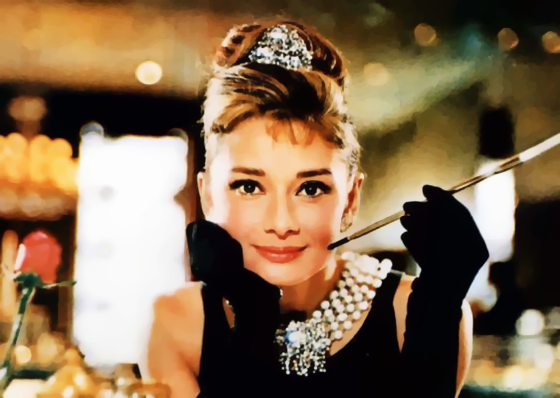
\includegraphics[width=\textwidth]{img/approximation/rof/01hepburn.png}
%                 \caption{$\lambda = 0.1$}
%             \end{subfigure}
%             \begin{subfigure}[b]{0.45\textwidth}
%                 \includegraphics[width=\textwidth]{img/approximation/rof/06hepburn.png}
%                 \caption{$\lambda = 0.6$}
%             \end{subfigure}
%             \begin{subfigure}[b]{0.45\textwidth}
%                 \includegraphics[width=\textwidth]{img/approximation/rof/09hepburn.png}
%                 \caption{$\lambda = 0.9$}
%             \end{subfigure}
%             \caption{Approximation of Audrey Hepburn with the ROF Model. The higher $\lambda$ the closer the outcome of the algrithm to the original image.}
%         \label{fig:rof_hepburn_compare}
%         \end{figure}
%     % subsection image_approximation_using_the_rof_model (end)
% % section image_approximation (end)

% \begin{figure}[ht]
%     \centering
%     \begin{subfigure}[b]{0.45\textwidth}
%         \includegraphics[width=\textwidth]{img/approximation/tvl1/06hepburn.png}
%         \caption{$\lambda = 0.6$}
%     \end{subfigure}
%     \begin{subfigure}[b]{0.45\textwidth}
%         \includegraphics[width=\textwidth]{img/approximation/tvl1/07hepburn.png}
%         \caption{$\lambda = 0.7$}
%     \end{subfigure}
%     \begin{subfigure}[b]{0.45\textwidth}
%         \includegraphics[width=\textwidth]{img/approximation/tvl1/08hepburn.png}
%         \caption{$\lambda = 0.8$}
%     \end{subfigure}
%     \begin{subfigure}[b]{0.45\textwidth}
%         \includegraphics[width=\textwidth]{img/approximation/tvl1/09hepburn.png}
%         \caption{$\lambda = 0.9$}
%     \end{subfigure}
%     \caption{Approximation of Audrey Hepburn with the TVL1 Model. The higher $\lambda$ the closer the outcome of the algrithm to the original image.}
% \label{fig:tvl1_hepburn_compare}
% \end{figure}

% \begin{figure}[ht]
%     \centering
%     \begin{subfigure}[b]{0.4\textwidth}
%         \includegraphics[width=\textwidth]{img/approximation/tvl1/06lena.png}
%         \caption{$\lambda = 0.6$}
%     \end{subfigure}
%     \begin{subfigure}[b]{0.4\textwidth}
%         \includegraphics[width=\textwidth]{img/approximation/tvl1/07lena.png}
%         \caption{$\lambda = 0.7$}
%     \end{subfigure}
%     \begin{subfigure}[b]{0.4\textwidth}
%         \includegraphics[width=\textwidth]{img/approximation/tvl1/08lena.png}
%         \caption{$\lambda = 0.8$}
%     \end{subfigure}
%     \begin{subfigure}[b]{0.4\textwidth}
%         \includegraphics[width=\textwidth]{img/approximation/tvl1/09lena.png}
%         \caption{$\lambda = 0.9$}
%     \end{subfigure}
%     \caption{Approximation of the Lena image with the TVL1 Model. Again, the higher $\lambda$ the closer the outcome of the algrithm to the original image.}
% \label{fig:tvl1_lena_compare}
% \end{figure}

% \begin{figure}[ht]
%     \centering
%     \begin{subfigure}[b]{0.45\textwidth}
%         \includegraphics[width=\textwidth]{img/approximation/realtime/003hepburn20.png}
%         \caption{$\alpha = 20, \lambda = 0.03$ (piecewise smooth)}
%     \end{subfigure}
%     \begin{subfigure}[b]{0.45\textwidth}
%         \includegraphics[width=\textwidth]{img/approximation/realtime/05hepburn500.png}
%         \caption{$\alpha = 500, \lambda = 0.5$ (piecewise constant)}
%     \end{subfigure}
%     \begin{subfigure}[b]{0.45\textwidth}
%         \includegraphics[width=\textwidth]{img/approximation/realtime/004hepburn20.png}
%         \caption{$\alpha = 20, \lambda = 0.04$ (piecewise smooth)}
%     \end{subfigure}
%     \begin{subfigure}[b]{0.45\textwidth}
%         \includegraphics[width=\textwidth]{img/approximation/realtime/07hepburn500.png}
%         \caption{$\alpha = 500, \lambda = 0.7$ (piecewise constant)}
%     \end{subfigure}
%     \caption{Approximation of Audrey Hepburn with the Mumford-Shah Model. The higher $\lambda$ the closer the outcome of the algrithm to the original image.}
% \label{fig:realtime_hepburn_compare}
% \end{figure}

% \begin{figure}[ht]
%     \centering
%     \begin{subfigure}[b]{0.4\textwidth}
%         \includegraphics[width=\textwidth]{img/approximation/realtime/003lena20.png}
%         \caption{$\alpha = 20, \lambda = 0.03$ (piecewise smooth)}
%     \end{subfigure}
%     \begin{subfigure}[b]{0.4\textwidth}
%         \includegraphics[width=\textwidth]{img/approximation/realtime/007lena500.png}
%         \caption{$\alpha = 500, \lambda = 0.5$ (piecewise constant)}
%     \end{subfigure}
%     \begin{subfigure}[b]{0.4\textwidth}
%         \includegraphics[width=\textwidth]{img/approximation/realtime/004lena20.png}
%         \caption{$\alpha = 20, \lambda = 0.04$ (piecewise smooth)}
%     \end{subfigure}
%     \begin{subfigure}[b]{0.4\textwidth}
%         \includegraphics[width=\textwidth]{img/approximation/realtime/008lena500.png}
%         \caption{$\alpha = 500, \lambda = 0.7$ (piecewise constant)}
%     \end{subfigure}
%     \caption{Approximation of the Lena image with the Mumford-Shah Model. Again, the higher $\lambda$ the closer the outcome of the algrithm to the original image.}
% \label{fig:realtime_lena_compare}
% \end{figure}

% \begin{figure}[ht]
%     \centering
%     \begin{center}
%         \rotatebox{90}{$\lambda = 0.005$}
%         \begin{subfigure}[b]{0.21\textwidth}
%             \includegraphics[width=\textwidth]{img/evolution/rof/0005hepburn.png}
%         \end{subfigure}
%         \rotatebox{90}{$\lambda = 0.2$}
%         \begin{subfigure}[b]{0.21\textwidth}
%             \includegraphics[width=\textwidth]{img/evolution/tvl1/02hepburn.png}
%         \end{subfigure}
%         \rotatebox{90}{$\lambda = 0.01$}
%         \begin{subfigure}[b]{0.21\textwidth}
%             \includegraphics[width=\textwidth]{img/evolution/realtime/001hepburn20.png}
%         \end{subfigure}
%         \rotatebox{90}{$\lambda = 0.1$}
%         \begin{subfigure}[b]{0.21\textwidth}
%             \includegraphics[width=\textwidth]{img/evolution/realtime/01hepburn500.png}
%         \end{subfigure}
%     \end{center}
%     \begin{center}
%         \rotatebox{90}{$\lambda = 0.007$}
%         \begin{subfigure}[b]{0.21\textwidth}
%             \includegraphics[width=\textwidth]{img/evolution/rof/0007hepburn.png}
%         \end{subfigure}
%         \rotatebox{90}{$\lambda = 0.3$}
%         \begin{subfigure}[b]{0.21\textwidth}
%             \includegraphics[width=\textwidth]{img/evolution/tvl1/03hepburn.png}
%         \end{subfigure}
%         \rotatebox{90}{$\lambda = 0.03$}
%         \begin{subfigure}[b]{0.21\textwidth}
%             \includegraphics[width=\textwidth]{img/evolution/realtime/003hepburn20.png}
%         \end{subfigure}
%         \rotatebox{90}{$\lambda = 0.3$}
%         \begin{subfigure}[b]{0.21\textwidth}
%             \includegraphics[width=\textwidth]{img/evolution/realtime/03hepburn500.png}
%         \end{subfigure}
%     \end{center}
%     \begin{center}
%         \rotatebox{90}{$\lambda = 0.009$}
%         \begin{subfigure}[b]{0.21\textwidth}
%             \includegraphics[width=\textwidth]{img/evolution/rof/0009hepburn.png}
%         \end{subfigure}
%         \rotatebox{90}{$\lambda = 0.4$}
%         \begin{subfigure}[b]{0.21\textwidth}
%             \includegraphics[width=\textwidth]{img/evolution/tvl1/04hepburn.png}
%         \end{subfigure}
%         \rotatebox{90}{$\lambda = 0.05$}
%         \begin{subfigure}[b]{0.21\textwidth}
%             \includegraphics[width=\textwidth]{img/evolution/realtime/005hepburn20.png}
%         \end{subfigure}
%         \rotatebox{90}{$\lambda = 0.5$}
%         \begin{subfigure}[b]{0.21\textwidth}
%             \includegraphics[width=\textwidth]{img/evolution/realtime/05hepburn500.png}
%         \end{subfigure}
%     \end{center}
%     \begin{center}
%         \rotatebox{90}{$\lambda = 0.02$}
%         \begin{subfigure}[b]{0.21\textwidth}
%             \includegraphics[width=\textwidth]{img/evolution/rof/002hepburn.png}
%         \end{subfigure}
%         \rotatebox{90}{$\lambda = 0.5$}
%         \begin{subfigure}[b]{0.21\textwidth}
%             \includegraphics[width=\textwidth]{img/evolution/tvl1/05hepburn.png}
%         \end{subfigure}
%         \rotatebox{90}{$\lambda = 0.07$}
%         \begin{subfigure}[b]{0.21\textwidth}
%             \includegraphics[width=\textwidth]{img/evolution/realtime/007hepburn20.png}
%         \end{subfigure}
%         \rotatebox{90}{$\lambda = 0.7$}
%         \begin{subfigure}[b]{0.21\textwidth}
%             \includegraphics[width=\textwidth]{img/evolution/realtime/07hepburn500.png}
%         \end{subfigure}
%     \end{center}
%     \begin{center}
%         \rotatebox{90}{$\lambda = 0.04$}
%         \begin{subfigure}[b]{0.21\textwidth}
%             \includegraphics[width=\textwidth]{img/evolution/rof/004hepburn.png}
%         \end{subfigure}
%         \rotatebox{90}{$\lambda = 0.6$}
%         \begin{subfigure}[b]{0.21\textwidth}
%             \includegraphics[width=\textwidth]{img/evolution/tvl1/06hepburn.png}
%         \end{subfigure}
%         \rotatebox{90}{$\lambda = 0.09$}
%         \begin{subfigure}[b]{0.21\textwidth}
%             \includegraphics[width=\textwidth]{img/evolution/realtime/009hepburn20.png}
%         \end{subfigure}
%         \rotatebox{90}{$\lambda = 0.9$}
%         \begin{subfigure}[b]{0.21\textwidth}
%             \includegraphics[width=\textwidth]{img/evolution/realtime/09hepburn500.png}
%         \end{subfigure}
%     \end{center}
%     \caption{Evolution of the Audrey Hepburn image, whereas the left column shows the ROF Model, the second column the TVL1 Model, the third column resembles the piecewise smooth approximation of the Mumford-Shah Model with the real-time minimizer with $\alpha = 20$. The right column shows the piecewise constant case of the last mentioned algorithm with $\alpha = 500$.}
% \end{figure}

% \begin{figure}[ht]
% \centering
% \begin{center}
%     \rotatebox{90}{$\lambda = 0.005$}
%     \begin{subfigure}[b]{0.19\textwidth}
%         \includegraphics[width=\textwidth]{img/evolution/rof/0005lena.png}
%     \end{subfigure}
%     \rotatebox{90}{$\lambda = 0.2$}
%     \begin{subfigure}[b]{0.19\textwidth}
%         \includegraphics[width=\textwidth]{img/evolution/tvl1/02lena.png}
%     \end{subfigure}
%     \rotatebox{90}{$\lambda = 0.01$}
%     \begin{subfigure}[b]{0.19\textwidth}
%         \includegraphics[width=\textwidth]{img/evolution/realtime/001lena20.png}
%     \end{subfigure}
%     \rotatebox{90}{$\lambda = 0.01$}
%     \begin{subfigure}[b]{0.19\textwidth}
%         \includegraphics[width=\textwidth]{img/evolution/realtime/001lena500.png}
%     \end{subfigure}
% \end{center}
% \begin{center}
%     \rotatebox{90}{$\lambda = 0.007$}
%     \begin{subfigure}[b]{0.19\textwidth}
%         \includegraphics[width=\textwidth]{img/evolution/rof/0007lena.png}
%     \end{subfigure}
%     \rotatebox{90}{$\lambda = 0.3$}
%     \begin{subfigure}[b]{0.19\textwidth}
%         \includegraphics[width=\textwidth]{img/evolution/tvl1/03lena.png}
%     \end{subfigure}
%     \rotatebox{90}{$\lambda = 0.03$}
%     \begin{subfigure}[b]{0.19\textwidth}
%         \includegraphics[width=\textwidth]{img/evolution/realtime/003lena20.png}
%     \end{subfigure}
%     \rotatebox{90}{$\lambda = 0.03$}
%     \begin{subfigure}[b]{0.19\textwidth}
%         \includegraphics[width=\textwidth]{img/evolution/realtime/003lena500.png}
%     \end{subfigure}
% \end{center}
% \begin{center}
%     \rotatebox{90}{$\lambda = 0.009$}
%     \begin{subfigure}[b]{0.19\textwidth}
%         \includegraphics[width=\textwidth]{img/evolution/rof/0009lena.png}
%     \end{subfigure}
%     \rotatebox{90}{$\lambda = 0.4$}
%     \begin{subfigure}[b]{0.19\textwidth}
%         \includegraphics[width=\textwidth]{img/evolution/tvl1/04lena.png}
%     \end{subfigure}
%     \rotatebox{90}{$\lambda = 0.05$}
%     \begin{subfigure}[b]{0.19\textwidth}
%         \includegraphics[width=\textwidth]{img/evolution/realtime/005lena20.png}
%     \end{subfigure}
%     \rotatebox{90}{$\lambda = 0.05$}
%     \begin{subfigure}[b]{0.19\textwidth}
%         \includegraphics[width=\textwidth]{img/evolution/realtime/005lena500.png}
%     \end{subfigure}
% \end{center}
% \begin{center}
%     \rotatebox{90}{$\lambda = 0.02$}
%     \begin{subfigure}[b]{0.19\textwidth}
%         \includegraphics[width=\textwidth]{img/evolution/rof/002lena.png}
%     \end{subfigure}
%     \rotatebox{90}{$\lambda = 0.5$}
%     \begin{subfigure}[b]{0.19\textwidth}
%         \includegraphics[width=\textwidth]{img/evolution/tvl1/05lena.png}
%     \end{subfigure}
%     \rotatebox{90}{$\lambda = 0.07$}
%     \begin{subfigure}[b]{0.19\textwidth}
%         \includegraphics[width=\textwidth]{img/evolution/realtime/007lena20.png}
%     \end{subfigure}
%     \rotatebox{90}{$\lambda = 0.07$}
%     \begin{subfigure}[b]{0.19\textwidth}
%         \includegraphics[width=\textwidth]{img/evolution/realtime/007lena500.png}
%     \end{subfigure}
% \end{center}
% \begin{center}
%     \rotatebox{90}{$\lambda = 0.04$}
%     \begin{subfigure}[b]{0.19\textwidth}
%         \includegraphics[width=\textwidth]{img/evolution/rof/004lena.png}
%     \end{subfigure}
%     \rotatebox{90}{$\lambda = 0.6$}
%     \begin{subfigure}[b]{0.19\textwidth}
%         \includegraphics[width=\textwidth]{img/evolution/tvl1/06lena.png}
%     \end{subfigure}
%     \rotatebox{90}{$\lambda = 0.09$}
%     \begin{subfigure}[b]{0.19\textwidth}
%         \includegraphics[width=\textwidth]{img/evolution/realtime/009lena20.png}
%     \end{subfigure}
%     \rotatebox{90}{$\lambda = 0.09$}
%     \begin{subfigure}[b]{0.19\textwidth}
%         \includegraphics[width=\textwidth]{img/evolution/realtime/009lena500.png}
%     \end{subfigure}
% \end{center}
% \caption{Evolution of the Lena image, whereas the left column shows the ROF Model, the second column the TVL1 Model, the third column resembles the piecewise smooth approximation of the Mumford-Shah Model with the real-time minimizer with $\alpha = 20$. The right column shows the piecewise constant case of the last mentioned algorithm with $\alpha = 500$.}
% \end{figure}